%%%%%%%%%%%%%%%%%%%%%%%%%%%%%%%%%%%%%%%%%%%%%%%%%%%%%%%%%%%%%%%%%%%%%%%%%%%%%%%
% Active Learning Machine Learning Methodology %%%%%%%%%%%%%%%%%%%%%%%%%%%%%%%%
% %%%%%%%%%%%%%%%%%%%%%%%%%%%%%%%%%%%%%%%%%%%%%%%%%%%%%%%%%%%%%%%%%%%%%%%%%%%%%
%
% Points to mention:
%    Voronoi is used because it is insensitive to volume expansions of structure
%    TODO: Explain PCA analysis
%    TODO: Get PCA reference
%
% TODO:
%    Why AB2 and AB3
%%%%%%%%%%%%%%%%%%%%%%%%%%%%%%%%%%%%%%%%%%%%%%%%%%%%%%%%%%%%%%%%%%%%%%%%%%%%%%%


% ################################# Paragraph #################################
% %%%%%%%%%%%%%%%%%%%%%%%%%%%%%%%%%%%%%%%%%%%%%%%%%%%%%%%%%%%%%%%%%%%%%%%%%%%%%
% General intro to AL scheme
% Basic gist, i.e. define our candidate space of materials to explore within
% (we do this by looking taking all structurally unique systems in DBs)
% To start the AL we take the few systems that have DFT calcs (more generally
% we can just choose random structures)
% We then build a surrogate model (GP, initially really bad) to predict the
% stability of the entire candidate space
% %%%%%%%%%%%%%%%%%%%%%%%%%%%%%%%%%%%%%%%%%%%%%%%%%%%%%%%%%%%%%%%%%%%%%%%%%%%%%
% | - Paragraph start
% Maybe "crystal structures" instead of "materials"? More to the point?
%CP: agree
Here, we present a machine-learning based methodology for discovering new stable and meta-stable crystal structures.
%
Our approach builds on the principles of surrogate active learning [Refs?],
where a model is iteratively trained on available DFT data.
%
The model predictions are used as a surrogate to the DFT energy evaluations,
which are used to acquire new systems for DFT in the population based on an acquisition criteria.
% Add the Hammer paper (R58) as another citation
Active learning in conjunction with genetic algorithms has been demonstrated to successfully speed up materials discovery for alloy nanoparticles \cite{Jennings2019}, and ...[Other refs?],  structural optimizations \cite{hansen2019atomistic}, and transition-state calculations \cite{torres2019low}.
% TEMP
The methodology consists of two steps (outlined in  \ref{fig:all_diagram}).
%
The first step is the generation of the candidate space,
which defines the inclusive list of all crystal structures to be screened through during the search routine.
%
Since the initial candidates determines which structures that can ultimately be discovered, it is crucial to define a candidate space that is sufficiently diverse.
% TEMP Say more
The second part of the algorithm is the iterative active learning algorithm.

% | - __old__
% Our machine learning accelerated materials discovery method proceeds through the following steps:
% First, the dataset of candidate materials is constructed.
% This data set will define the totality of materials that will be considered by the search algorithm,
% this is done because the search space of materials is not a continous space but a discrite array of individual structures.
% Next, the dataset of materials is transformed into a vectorial representation by using a fingerprinting method that encodes the relevent chemical and structural information.
% __|

% __|


% ################################# Paragraph #################################
% %%%%%%%%%%%%%%%%%%%%%%%%%%%%%%%%%%%%%%%%%%%%%%%%%%%%%%%%%%%%%%%%%%%%%%%%%%%%%
% !!!!!!!!!! NEW PARAGRAPH !!!!!!!!!! Can I get all of the methodology here
% %%%%%%%%%%%%%%%%%%%%%%%%%%%%%%%%%%%%%%%%%%%%%%%%%%%%%%%%%%%%%%%%%%%%%%%%%%%%%
% | - Paragraph start
% TODO Ask @Ankit for these numbers
% The MP project number should be correct, but the OQMD number might be wrong
% MP{AB2: 3995, AB3: 2849} | OQMD{AB2: 533, AB3:20915}
In Schema \ref{fig:all_diagram} we show the {\bf overall process with the integrated active learning loop}. {\bf We start with ...}.
%
{\bf We continue with  with XXX...}
%
The structures that comprise the candidate data sets for \IrOtwo and \IrOthree were constructed by parsing for all bulk \ABtwo and \ABthree structures in both the Materials Project\cite{Jain2013} and OQMD\cite{Kirklin2015} databases
(in total 4528 \ABtwo and 23764 \ABthree entries).
%
Structurally redundant systems were then removed via a space-group based structural classification scheme developed by Jain et al. \cite{Jain2018}.
%
The resulting data set is composed of 697 \ABtwo and 259 \ABthree structural prototypes for which iridium and oxygen were replaced for the A and B sites, respectively.
%
Finally, a coarse isotropic volume relaxation was performed to accommodate for the difference in atomic radii of Ir and O to the elements that originally comprised the structure in OQMD/MP.
%
Additional details about our method can be found in the SI.
% TODO Double check numbers
Only candidates that were successfully optimized with DFT were ultimately included so that the model could be properly validated,
which gives a final candidate data set of 448 and 258 \ABtwo and \ABthree structurally unique polymorphs.
%
While size of this dataset is not particularly large, it will serve the purpose of demonstrating the polymorph discovery routine as a proof of concept.
%
Additionally, the dataset is small enough that computing all of the structural candidats with ab-initio DFT is tractable, thus allowing us to validate the performance of the model.
% __|


% ################################# Paragraph #################################
% %%%%%%%%%%%%%%%%%%%%%%%%%%%%%%%%%%%%%%%%%%%%%%%%%%%%%%%%%%%%%%%%%%%%%%%%%%%%%
% !!!!!!!!!! NEW PARAGRAPH !!!!!!!!!! Can I get all of the methodology here
% %%%%%%%%%%%%%%%%%%%%%%%%%%%%%%%%%%%%%%%%%%%%%%%%%%%%%%%%%%%%%%%%%%%%%%%%%%%%%
% | - Paragraph start
The candidate data set was featurized using the Voronoi tessellation fingerprinting scheme developed by Ward et al. \cite{Ward2017} which produces a 271 feature vector for each material that are insensitive to isotropic expansions and contractions in a crystals lattice.
% How many columns of the 271 are redundant if stoich and composition are frozen
Herein, we apply our active learning model to the \IrOtwo and \IrOthree spaces separately, because we are interested in the most stable polymorphs at each stoichiometry. Constraining the candidate space to having uniform stoichiometry reduces the 271 feature vector to 101 non-zero variance features, thus reducing the dimensionality of our problem significantly.
% COMBAK
Further dimensionality reduction is achieved via a principle component analysis (PCA) \cite{Tipping1999}, which was used to reduce the remaining 101 features to 11.
%
The active learning algorithm proceeds through iterative generations of ML training, prediction, and acquisition steps that are visualized in figure \ref{fig:iro2_al}.
% COMBAK Did I get all of the important features of GP here? @Jose
To start, Gaussian process (GP) regression is used to train a regression model on a small seed set of DFT formation energies from randomly selected structures in the candidate space.
%
The model is then used to predict the formation energies of the entire candidate space.
%
Following this, the predictions are used to determine which systems to acquire, by minimizing the so-called GP-UCB acquisition function:
% The name for this kind of acquisition is calld GP-UCB (Upper confidence bound)
% https://www.cse.wustl.edu/~garnett/cse515t/spring_2015/files/lecture_notes/12.pdf
\begin{equation}
    U = \mu - \kappa \sigma,
\end{equation}
%
where $\mu$ and $\sigma$ is the predicted mean and standard deviation of the formation energy,
and $\kappa$ is a free parameter to tune the relative weighting between exploiting low formation energy systems (small $\kappa$) and exploring high uncertainty regions of the candidate space (large $\kappa$).
%
In this work we attempt to trade off exploitation and exploration by weighting the predicted formation energy and the associated uncertainty to bias systems that are both low energy and high uncertainty.
%
Here, $\kappa$ is set to $1$ which equally weights the energy and uncertainty.
% TODO N is used into mean number of atoms (FIX)
Once ranked, the N systems that minimize the acquisition function are selected for full DFT calculations, which are included in the training data of subsequent AL generations.
% COMBAK We are discussing alternative convergence criteria, or whether to even
% have convergence criteria here
The AL loop proceeds until convergence is achieved, which here is chosen to be the generation at which the structures within the range of metastability, here taken as 0.1 eV/atom, are unchanging over three consecutive generations.
% __|



% | - Figure | Active Learning Algorithm **************************************
\begin{figure*}[!htb]
\centering
\makebox[\textwidth][c]{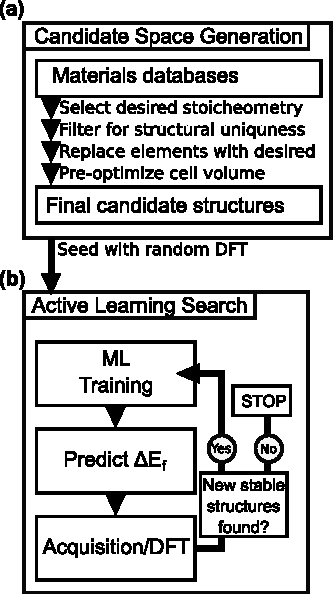
\includegraphics
  {02_figures/al_diagram/Surrogate_model_mine.pdf}
  }
\caption{\label{fig:all_diagram}
% Probably better to keep this caption really concise and refer to the text
Process flow diagram for the active learning accelerated algorithm. The procedure is composed of (a) generation of the candidate set of considered crystal structures constructed from DFT materials databases and (b) iterative active learning surrogate search of the candidate space.
}
\end{figure*}
% __|



% | - TRANSFER THIS TO SI AND MAKE SURE IT'S NOT TOO REDUNDANT WITH MAIN TEXT
%  are used as the regression model because they are highly flexible and can quantify the uncertainty of their predictions (see SI for details on the GP methodology).
% %
% The uncertainty quantification is used by the aquisition criteria which ranks the fitness of each prediction by weight both the predicted formation energy and the uncertainty assocated with the prediction as shown in equation TEMP.

% % ################################# Paragraph #################################
% % %%%%%%%%%%%%%%%%%%%%%%%%%%%%%%%%%%%%%%%%%%%%%%%%%%%%%%%%%%%%%%%%%%%%%%%%%%%%%
% % Data prep. | Unique Structures | Atom subst., V relax | Fingerprinting
% % Shift most of this to the SI and keep it simple instead
% % %%%%%%%%%%%%%%%%%%%%%%%%%%%%%%%%%%%%%%%%%%%%%%%%%%%%%%%%%%%%%%%%%%%%%%%%%%%%%
% % | - Paragraph start
% The structures that comprise the candidate data set were constructed by parsing for structurally unique systems in the OQMD and Materials Project DFT databases.
% %
% The structural uniqueness was performed using a space-group symmetry classification scheme developed by Jain et al. \cite{Jain2018},
% which can classify a structure based on its composition and structure.
%  (see SI for more details on the structural classification scheme).
% %
% This structural classification scheme can directly serve as a structural fingerprint and has successfully been applied towards the prediction of formation energies of inorganic compounds \cite{Jain2018}
% %
% To focus the scope of the study, only \ABtwo  and \ABthree stoichiometries were parsed from the databases.
% %
% Additionally, only structures with less than 75 atoms per unit cell were considered because
% 1.) they would be computationally prohibitive to simmulate with DFT and
% 2.) large unit cells are less likely to form well-ordered crystalline phase and/or more likely to relax into crystal structures that can be represented in smaller cells.
% %
% The \ABtwo formula was chosen because it includes \rIrOtwo, the known most stable polymorph of \IrOtwo.
% %
% Importantly, \ABthree was chosen to include high valency \IrOthree structures in our search.
% %
% The results of the classification scheme resulted in a XYZ AB2 and XYZ AB3 structural prototypes for which iridium and oxygen were replaced for A and B sites, respectively.
% %
% Finally, a coarse isotropic volume relaxation based on atomic radii was performed on the structures to accommodate the atomic radii of iridium and oxygen into the lattice.
% %
% Finally, a Voronoi tessellation based fingerprinting scheme developed by Ward et al. \cite{Ward2017} was used to encode the relevant chemical information for each structure into a vector quantity of length 271.
% %
% The Voronoi based method was used because it is insensitive to volume relaxation.
% %
% Separate, independent models were used for \IrOtwo and \IrOthree to reduce the complexity of the space, this has the additional effect of making a large number of the fingerprint descriptors redundant.
% % How many columns of the 271 are redundant if stoich and composition are frozen
% As a result, the 271 length feature space is reduced to a TEMP length vector.
% %
% PCA was used to reduce the dimensionality of the feature space from 271 to 20 features such that 99 \% of the variance is captured \cite{Tipping1999}.
% % __|
%
%
% % ################################# Paragraph #################################
% % %%%%%%%%%%%%%%%%%%%%%%%%%%%%%%%%%%%%%%%%%%%%%%%%%%%%%%%%%%%%%%%%%%%%%%%%%%%%%
% % Iterative Training of Gaussian Process
% % TODO go through fingerprinting here, not previous part
% % %%%%%%%%%%%%%%%%%%%%%%%%%%%%%%%%%%%%%%%%%%%%%%%%%%%%%%%%%%%%%%%%%%%%%%%%%%%%%
% % | - Paragraph start
% The active learning algorithm proceeds through iterative ML training, prediction, and acquisition steps and is visualized in figure TEMP.
% %
% While any regression technique can be used, we employed the Gaussian process (GP) regression model because it offers a high degree of flexibility and, most importantly, built-in uncertainty quantification.
% % TODO: Does the acquisition function we use have a name?
% Uncertainty quantification on the predicted formation energies is important because its used in the acquisition criteria.
% %
% Further details on the GP model, including hyper parameter information, is including in the SI.
% %
% The acquisition is made by selecting the $N$ systems with the lowest value of the acquisition function.
% %
% The acquisition function is defined in terms of the predicted formation energy, E, and the uncertainty, U:
%
% \begin{equation}
%     F = E - \kappa U,
% \end{equation}
%
% where the parameter $\kappa$ can be tuned to probe low uncertainty (small $\kappa$) or high uncertainty regions  (large $\kappa$).
% % TODO: Write aquisition function here, again does it have a name
% %$a = b + c$
% %
% The value of $N$ determines how many structures are selected for DFT calculations,
% and as such, determines the degree of parallization of the routine. The optimal value of $N$ depends on the computational resources available, as small values of N result in an algorithm that is slow, as every DFT calculation is performed serially.
% % TODO: Is this statement true?
% Larger values of N speed up the active-learning algorithm, but leads to a higher number of DFT calculations performed before convergence. %but potentially decreases the efficiency of the algorithm by TEMP TEMP.
% %
% Here we chose a value $N=10$.
% %
% The acquired structures are initially volume relaxed, followed by a full relaxation of all of the atomic coordinates,
% see SI for additional details on the DFT methodology.
% % This is wordy
% The AL loop proceeds until convergence is achieved, which here is defined as the point at which %the model has determined the lowest $N$ structures and has achieved a degree of accuracy for the candidate space such that
% no structures have predicted formation energies with an uncertainty bound lower than the most stable $N$ structures.
% % __|

% __|
